\vspace*{-4ex}

En üst düzey teknolojik alt yapısıyla Türkiye’de bir ilk olan Sabancı Üniversitesi Altunizade Dijital Kampüs; teknoloji, iş dünyası ve akademiyi birleştiren bir odak noktasıdır.
Yenilikçi bir eğitim anlayışıyla oluşturulan Sabancı Üniversitesi Altunizade Dijital Kampüs, öğrencilere gerek sınıfın içinde gerekse dünyanın diledikleri yerinden bağlanarak en
iyi eğitimi alma imkanı sunmaktadır. Dijital Kampüs’te yer alan tüm sınıflar Hyflex teknolojisine sahiptir.
Öğrencilerimiz programlara Hyflex teknolojisi sayesinde birebir ya da sınıftaymış hissi yaratan bir dijital ortamla bulundukları yerden katılabilmektedirler.

Dijital Kampüs, öğrencilerimizin bireysel olarak veya gruplar halinde çalışabileceği ve iş dünyası temsilcileri ile buluşabileceği, projeler üretebileceği ve geliştirebileceği eşsiz bir altyapıya ev sahipliği yapmaktadır.
Dijital Kampüs’te yüksek teknik donanıma sahip 9 hibrit sınıf, 2 profesyonel kayıt stüdyosu, 2 grup çalışma odası, bilimsel showroom, konferans salonu, dinlenme ve yemek salonları bulunmaktadır.

\textbf{Altunizade Dijital Kampüs'e Ulaşım:} Küçük Çamlıca Mahallesi Şehit İsmail Moray Sokak No:3 Kısıklı/Altunizade, 34696, Üsküdar/İstanbul

\begin{itemize}
  \setlength{\itemsep}{0pt}
  \setlength{\parskip}{0pt}
	\item Üsküdar / Çekmeköy M5 metro ile Altunizade indikten sonra 2 numaralı çıkış takip edildikten sonra kampüs hemen yanıdır.
	\item Metrobüs ile de Altunizade durağında indikten sonra tam karşınızda bulunmaktadır.
\end{itemize}

\begin{figure}
\centering
\vspace*{-8ex}
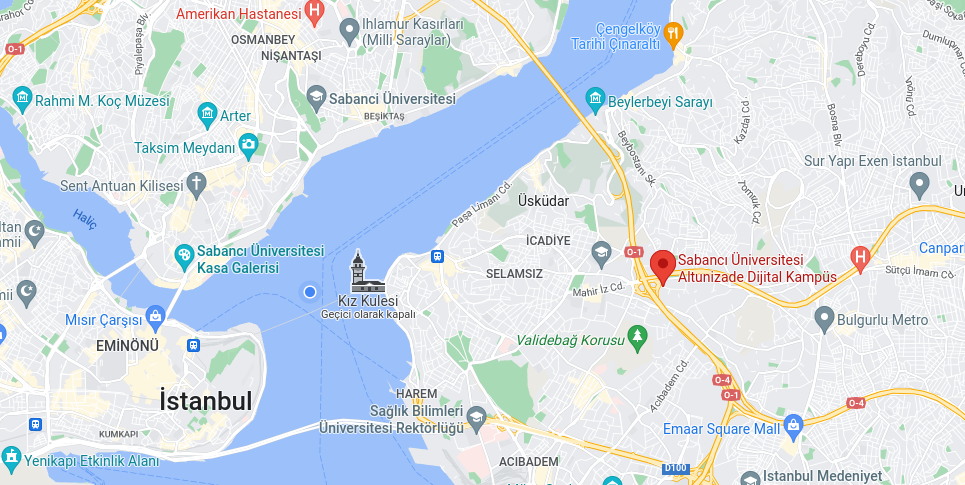
\includegraphics[width=0.95\textwidth]{altunizade_2.png}
\end{figure}
